\documentclass{beamer}
\usepackage[utf8]{inputenc}
\usepackage[T1]{fontenc}
\usepackage{amsmath, amssymb, amsthm}
\usepackage{lmodern}
\usepackage{graphicx}
\usepackage{xcolor}
\usepackage{colortbl}
\usepackage{booktabs}
\usepackage{multirow}
\usepackage{array}

\usetheme{Madrid}
\usecolortheme{seahorse}

% Özel renk tanımları
\definecolor{deepblue}{RGB}{0,0,139}
\definecolor{deepred}{RGB}{139,0,0}
\definecolor{deepgreen}{RGB}{0,100,0}
\definecolor{myyellow}{RGB}{255,215,0}

\title{Wilson Teoremi, Fermat'ın Küçük Teoremi ve Euler-Fermat Teoremi}
\author{Barbaros Biçer}
\institute{Matematik ve Bilgisayar Bilimleri Bölümü}
\date{26 Haziran 2025}

% Özel blok stilleri
\setbeamercolor{block title}{fg=white,bg=deepblue}
\setbeamercolor{block body}{fg=black,bg=blue!10}
\setbeamercolor{alerted text}{fg=deepred}
\setbeamercolor{example text}{fg=deepgreen}

\begin{document}

\begin{frame}
  \titlepage
  \begin{center}
    
\includegraphics[width=0.3\textwidth]{university_logo.png} 
  \end{center}
\end{frame}

\begin{frame}{Sunum Planı}
  \tableofcontents
\end{frame}

\section{Wilson Teoremi}

\begin{frame}{Wilson Teoremi — Tarihsel Gelişim}
  \begin{block}{Kronolojik Bilgiler}
    \begin{itemize}
      \item 18. yüzyılın ortalarında, \textbf{John Wilson} adlı bir hukuk öğrencisi asal sayılarla ilgili bu dikkat çekici sonucu dile getirmiştir.
      \item Fakat bu teoremin ispatı, 1771 yılında \textbf{Joseph-Louis Lagrange} tarafından yapılmıştır. Bu, o dönem için oldukça önemli bir ilerlemedir.
      \item \textbf{Leibniz} gibi dönemin önemli matematikçileri bu sonucu daha önceden biliyor olsa da yayınlamamışlardır.
      \item Bu nedenle teorem, aslında ispatını yapmayan \textbf{Wilson}'ın adıyla anılır.
    \end{itemize}
  \end{block}
  
  \begin{alertblock}{İlginç Not}
    Wilson bu teoremi ispatlamamış olsa da, teorem onun adıyla anılmaktadır.
  \end{alertblock}
\end{frame}

\begin{frame}{Wilson Teoremi — Tanım ve Mantık}
  \begin{theorem}[Wilson Teoremi]
    Eğer $p$ asal sayı ise:
    \[
      (p - 1)! \equiv -1 \mod p
    \]
  \end{theorem}
  
  \begin{itemize}
    \item $(p-1)!$ ifadesi, $1$'den $(p-1)$'e kadar olan sayıların çarpımıdır.
    \item Modüler aritmetikte asal sayılar altında her elemanın bir çarpma tersi vardır.
    \item Sadece $1$ ve $p-1$ kendilerinin tersidir: $a^2 \equiv 1 \mod p$
    \item Diğer tüm sayılar tersleriyle eşleşir ve sadeleşir.
  \end{itemize}
\end{frame}

\begin{frame}{Wilson Teoremi — Mantığın Detayları}
  \begin{block}{Temel Fikir}
    Asal sayı $p$ için, $1, 2, ..., p-1$ sayılarını düşün. Bunlar $\mathbb{Z}_p^\times$ kümesinde yer alır ve hepsinin çarpma tersi vardır.
  \end{block}
  
  \begin{itemize}
    \item Her $a$ için bir $a^{-1}$ vardır ki: $a \cdot a^{-1} \equiv 1 \mod p$
    \item Ancak sadece $1$ ve $p-1$ kendi tersleridir çünkü:
    \[
    a^2 \equiv 1 \mod p \Rightarrow a \equiv \pm 1 \mod p
    \]
    \item Diğer tüm sayılar birbirleriyle eşleşerek sadeleşir.
    \item Geriye sadece $1 \cdot (p-1)$ kalır → Bu da $p-1 \equiv -1 \mod p$
  \end{itemize}
\end{frame}

\begin{frame}{Wilson Teoremi — Sezgisel Açıklama}
  \begin{exampleblock}{Örnek Bakış Açısı}
    \begin{itemize}
      \item $(p-1)!$ çarpımı: $1 \cdot 2 \cdot 3 \cdots (p-1)$
      \item $2$ ile $x$, $3$ ile $y$, $\dots$ gibi ters çiftler var.
      \item Tüm ters çiftler çarpıldığında sonuç hep $1$ olur.
      \item Sadece $1$ ve $p-1$ kalır → $1 \cdot (p-1) \equiv -1 \mod p$
    \end{itemize}
  \end{exampleblock}
\end{frame}

\begin{frame}{Wilson Teoremi — İspat}
  \begin{proof}
    \begin{itemize}
      \item $p$ asal ise, $\mathbb{Z}_p^\times = \{1, 2, ..., p-1\}$ bir çarpma grubudur.
      \item Bu gruptaki her elemanın bir çarpma tersi vardır.
      \item Yalnızca $1$ ve $p - 1$ kendilerinin tersidir.
      \item Geri kalanlar tersleriyle eşleşip çarpımları $1$ olur.
      \item O hâlde:
      \[
      (p - 1)! \equiv 1 \cdot (p - 1) \equiv p - 1 \equiv -1 \mod p
      \]
    \end{itemize}
  \end{proof}
\end{frame}

\begin{frame}{Örnek 1 — Wilson Teoremi Uygulaması}
  \textbf{Soru:} $p = 11$ için Wilson Teoremi'ni doğrulayın.
  
  \begin{solution}
  \begin{align*}
    10! &= 1 \cdot (2 \cdot 6) \cdot (3 \cdot 4) \cdot (5 \cdot 9) \cdot (7 \cdot 8) \cdot 10 \\
        &\equiv 1 \cdot (12) \cdot (12) \cdot (45) \cdot (56) \cdot 10 \mod 11 \\
        &\equiv 1 \cdot 1 \cdot 1 \cdot 1 \cdot 1 \cdot 10 \mod 11 \\
        &\equiv 10 \mod 11 \\
        &\equiv -1 \mod 11
  \end{align*}
  \end{solution}
  
  \begin{exampleblock}{Yorum}
    $10!$ mod 11 hesabında, tersler eşleştirildiği için geriye sadece $10$ kalır ve bu $-1$'e denktir.
  \end{exampleblock}
\end{frame}

\begin{frame}{Wilson Teoremi ve Asallık Testi}
  \begin{itemize}
    \item $(n - 1)! \equiv -1 \mod n$ ifadesi, yalnızca $n$ asal olduğunda geçerlidir.
    \item Bu ifade \textbf{hem gerekli hem de yeterlidir} — yani tersi de geçerlidir.
    \item Teorik olarak asal sayıları tanımlamakta kullanılabilir.
  \end{itemize}
  
  \begin{alertblock}{Pratikteki Sınırlamalar}
    \begin{itemize}
      \item Büyük sayılar için $(n - 1)!$ çok büyük olacağından, hesaplaması zordur.
      \item $n=10^6$ için $(n-1)!$ yaklaşık $5.5 \times 10^{5,565,708}$ basamaklıdır!
    \end{itemize}
  \end{alertblock}
\end{frame}

\begin{frame}{Yeni Nesil Soru — Uygulama}
  \textbf{Soru:}\\[0.5em]
  Bir şifreleme sistemi, asal sayıların $(p - 1)! \equiv -1 \mod p$ özelliğini kullanıyor. Buna göre, aşağıdakilerden hangisi bu sistemde kullanılabilir?

  \begin{itemize}
    \item[A)] 8
    \item[B)] 10
    \item[C)] 13
    \item[D)] 15
  \end{itemize}
  
  \pause
  \begin{solution}
  \begin{itemize}
    \item A, B ve D asal değildir → elenir.
    \item C için: $12! \equiv -1 \mod 13$ olur (Wilson Teoremi).
    \item \textbf{Doğru Cevap:} \alert{C) 13}
  \end{itemize}
  \end{solution}
\end{frame}

\section{Fermat'ın Küçük Teoremi}

\begin{frame}{Fermat'ın Küçük Teoremi — Tarihsel Arka Plan}
  \begin{columns}
    \column{0.6\textwidth}
    \begin{itemize}
      \item \textbf{Pierre de Fermat}, 1640 yılında teoremi Frenicle de Bessy'ye mektupla iletti.
      \item "Bu teoremin ispatı kısa ama yazmaya vaktim yok" diyerek detay vermedi.
      \item \textbf{Leonhard Euler}, 1736'da bu teoremin ilk ispatını yayımlamıştır.
      \item \textbf{Çinli matematikçiler}, $a = 2$ özel durumunu M.Ö. 500'lü yıllarda kullanıyordu.
    \end{itemize}
    
    \column{0.4\textwidth}
    \begin{figure}
      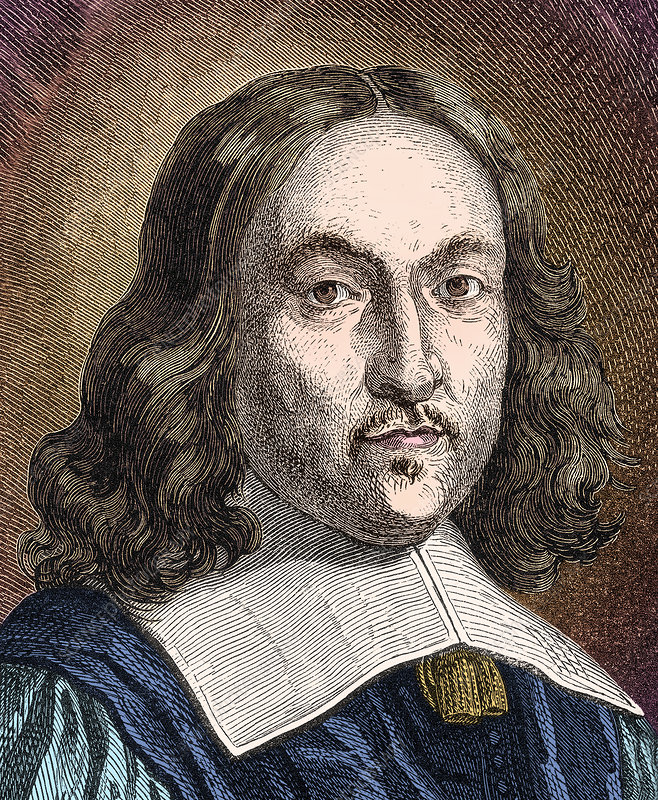
\includegraphics[width=\columnwidth]{fermat.jpg} % Kendi resim dosyanızı ekleyin
      \caption{Pierre de Fermat (1607-1665)}
    \end{figure}
  \end{columns}
\end{frame}

\begin{frame}{Fermat'ın Küçük Teoremi — Tanım}
  \begin{theorem}[Fermat'ın Küçük Teoremi]
    Eğer $p$ asal ve $a \not\equiv 0 \mod p$ ise:
    \[
      a^{p - 1} \equiv 1 \mod p
    \]
  \end{theorem}
  
  \begin{block}{Alternatif Form}
    $p$ asal ise her $a$ tamsayısı için:
    \[
      a^p \equiv a \mod p
    \]
  \end{block}
  
  \begin{itemize}
    \item Bu teorem, modüler aritmetikte üstel ifadelerin düzenini tanımlar.
    \item Asal sayı testleri ve kriptografi gibi alanlarda kullanılır.
  \end{itemize}
\end{frame}

% ✅ EKLENEN KISIM: WILSON BAĞLANTISI

\begin{frame}{Fermat'ın Küçük Teoremi — Wilson Teoremi ile Bağlantı}
  \begin{itemize}
    \item Fermat'ın teoremi de modüler aritmetiğin yapısına dayanır.
    \item Wilson Teoremi, $(p-1)! \equiv -1 \mod p$ ile asal sayıların modüler yapıdaki özelliğini gösterir.
    \item Fermat Teoremi'nde bu yapı, üs alma işlemi üzerinden kendini gösterir.
  \end{itemize}

  \begin{exampleblock}{Permütasyon Mantığı}
    \[
      a \cdot 2a \cdot 3a \cdots (p-1)a \equiv a^{p-1} \cdot (p-1)! \mod p
    \]
    \[
      \Rightarrow a^{p - 1} \cdot (p - 1)! \equiv (p - 1)! \mod p \Rightarrow a^{p-1} \equiv 1 \mod p
    \]
    Burada $(p-1)!$ sadeleşti çünkü tersliğini Wilson Teoremi sağladı.
  \end{exampleblock}
\end{frame}

\begin{frame}{Mantık — Permütasyon Yaklaşımı}
  \begin{itemize}
    \item $a, 2a, 3a, \dotsc, (p-1)a$ mod $p$ altında bir permütasyon oluşturur.
    \item Bunların çarpımı:
    \[
      a^{p - 1} \cdot (p - 1)! \equiv (p - 1)! \mod p
    \]
    \item Wilson Teoremi'ne göre $(p-1)! \equiv -1 \mod p$ ve sadeleştirilince:
    \[
      a^{p - 1} \equiv 1 \mod p
    \]
  \end{itemize}
\end{frame}

\begin{frame}{Örnek 1 — $12^6 \mod 7$}
  \begin{itemize}
    \item $12 \equiv 5 \mod 7$
    \item Fermat'ya göre ($p=7$):
    \[
      5^6 \equiv 1 \mod 7
    \]
    \item Doğrulama:
    \begin{align*}
      5^2 &= 25 \equiv 4 \mod 7 \\
      5^4 &= (5^2)^2 \equiv 4^2 = 16 \equiv 2 \mod 7 \\
      5^6 &= 5^4 \cdot 5^2 \equiv 2 \cdot 4 = 8 \equiv 1 \mod 7
    \end{align*}
  \end{itemize}
\end{frame}

\begin{frame}{Örnek 2 — $24^{1947} \mod 17$}
  \begin{itemize}
    \item $24 \equiv 7 \mod 17$
    \item Fermat'ya göre ($p=17$): $7^{16} \equiv 1 \mod 17$
    \item Üsü ayırma:
    \[
      1947 = 121 \cdot 16 + 11 \Rightarrow 7^{1947} = (7^{16})^{121} \cdot 7^{11} \equiv 1^{121} \cdot 7^{11} \mod 17
    \]
    \item $7^{11}$ hesaplaması:
    \begin{align*}
      7^2 &= 49 \equiv 15 \mod 17 \\
      7^4 &\equiv 15^2 = 225 \equiv 4 \mod 17 \\
      7^8 &\equiv 4^2 = 16 \equiv -1 \mod 17 \\
      7^{11} &= 7^8 \cdot 7^2 \cdot 7 \equiv (-1) \cdot 15 \cdot 7 = -105 \equiv 3 \mod 17
    \end{align*}
    \item Sonuç: $24^{1947} \equiv 3 \mod 17$
  \end{itemize}
\end{frame}

\begin{frame}{Ekstra Örnek — $17^{100} \mod 19$}
  \begin{itemize}
    \item $p = 19 \Rightarrow 17^{18} \equiv 1 \mod 19$
    \item Üsü ayırma:
    \[
      100 = 5 \cdot 18 + 10 \Rightarrow 17^{100} \equiv 17^{10} \mod 19
    \]
    \item Küçük üslerle hesap:
    \begin{align*}
      17^2 &= 289 \equiv 4 \mod 19 \\
      17^4 &\equiv 4^2 = 16 \mod 19 \\
      17^8 &\equiv 16^2 = 256 \equiv 9 \mod 19 \\
      17^{10} &= 17^8 \cdot 17^2 \equiv 9 \cdot 4 = 36 \equiv 17 \mod 19
    \end{align*}
    \item Sonuç: $17^{100} \equiv 17 \mod 19$
  \end{itemize}
\end{frame}

\begin{frame}{Fermat ile Ters Hesaplama}
  \begin{block}{Ters Bulma}
    Fermat'ın Küçük Teoremi'ne göre:
    \[
      a^{-1} \equiv a^{p-2} \mod p \quad \text{(p asal)}
    \]
  \end{block}
  
  \begin{exampleblock}{Örnek: $12^{-1} \mod 7$}
    \begin{itemize}
      \item $12 \equiv 5 \mod 7$
      \item $5^{-1} \equiv 5^{5} \mod 7$ ($p-2=5$)
      \item Hesaplama:
      \begin{align*}
        5^2 &\equiv 4 \mod 7 \\
        5^4 &\equiv 4^2 = 16 \equiv 2 \mod 7 \\
        5^5 &= 5^4 \cdot 5 \equiv 2 \cdot 5 = 10 \equiv 3 \mod 7
      \end{align*}
      \item Doğrulama: $5 \cdot 3 = 15 \equiv 1 \mod 7$
    \end{itemize}
  \end{exampleblock}
\end{frame}

\begin{frame}{Fermat'ın Özel Durumu — Çinli Matematikçiler}
  \begin{block}{Tarihsel Bilgi}
    Çinli matematikçiler, Han Hanedanı döneminde (M.Ö. 200) Fermat'ın $a = 2$ özel durumunu kullanıyordu:
    \[
      2^{p - 1} \equiv 1 \mod p
    \]
  \end{block}

  \begin{itemize}
    \item Bu yaklaşım, Çin Asallık Testi'nin temelini oluşturmuştur.
    \item Örneğin $p=7$ için:
    \[
      2^6 = 64 \equiv 1 \mod 7
    \]
  \end{itemize}
\end{frame}

\section{Euler-Fermat Teoremi}

\begin{frame}{Leonhard Euler — Kısa Biyografi}
  \begin{columns}
    \column{0.6\textwidth}
    \begin{itemize}
      \item 1707-1783 yılları arasında yaşamış İsviçreli matematikçi
      \item Matematiğin hemen her alanında katkı sağlamıştır
      \item Görme yetisini kaybetmesine rağmen üretkenliğini sürdürmüştür
      \item Fermat'ın Küçük Teoremi'ni genelleştirmiştir
    \end{itemize}
    
    \column{0.4\textwidth}
    \begin{figure}
      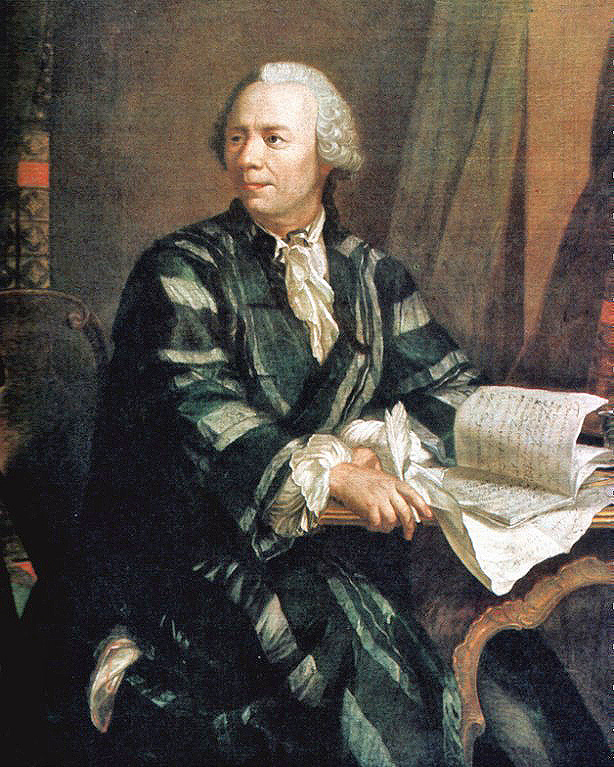
\includegraphics[width=\columnwidth]{euler.jpg} % Kendi resim dosyanızı ekleyin
      \caption{Leonhard Euler (1707-1783)}
    \end{figure}
  \end{columns}
\end{frame}

\begin{frame}{Euler'in Phi Fonksiyonu — Tanım}
  \begin{definition}[Euler Totient Fonksiyonu]
    $\varphi(n)$: $n$'den küçük ve $n$ ile aralarında asal olan sayıların sayısıdır.
  \end{definition}
  
  \begin{exampleblock}{Örnekler}
    \begin{itemize}
      \item $\varphi(4) = 2$ (1, 3)
      \item $\varphi(9) = 6$ (1, 2, 4, 5, 7, 8)
      \item $\varphi(12) = 4$ (1, 5, 7, 11)
      \item Eğer $p$ asal ise $\varphi(p) = p - 1$
    \end{itemize}
  \end{exampleblock}
\end{frame}

\begin{frame}{Phi Fonksiyonunun Özellikleri}
  \begin{block}{Çarpımsallık}
    $\gcd(m, n) = 1$ ise $\varphi(mn) = \varphi(m) \cdot \varphi(n)$
  \end{block}
  
  \begin{block}{Asal Kuvvetler}
    $\varphi(p^k) = p^k - p^{k - 1} = p^{k-1}(p-1)$
  \end{block}
  
  \begin{block}{Genel Formül}
    $n = p_1^{k_1}p_2^{k_2}\cdots p_r^{k_r}$ ise:
    \[
      \varphi(n) = n \left(1 - \frac{1}{p_1}\right)\left(1 - \frac{1}{p_2}\right)\cdots\left(1 - \frac{1}{p_r}\right)
    \]
  \end{block}
\end{frame}

\begin{frame}{Euler-Fermat Teoremi — Tanım}
  \begin{theorem}[Euler-Fermat Teoremi]
    Eğer $\gcd(a, n) = 1$ ise:
    \[
      a^{\varphi(n)} \equiv 1 \mod n
    \]
  \end{theorem}
  
  \begin{itemize}
    \item Fermat'ın Küçük Teoremi'nin genelleştirilmiş halidir.
    \item Modül asal olmasa da çalışır.
    \item Kriptografide (özellikle RSA'da) önemli uygulamaları vardır.
  \end{itemize}
\end{frame}


\begin{frame}{Euler-Fermat Teoremi — Fermat’tan Genelleme}
  \begin{itemize}
    \item Fermat Teoremi sadece asal sayılar için geçerlidir.
    \item Euler bu yapıyı genelleştirmiştir: modül asal olmak zorunda değildir.
    \item Fermat’ta: $\varphi(p) = p - 1$ olduğu için:
    \[
      a^{p - 1} \equiv 1 \mod p
    \]
    \item Euler: Eğer $n$ asal değilse bile, $a$ ile $n$ aralarında asal ise:
    \[
      a^{\varphi(n)} \equiv 1 \mod n
    \]
    \item Böylece tüm pozitif tam sayılar için genelleme yapılmış oldu.
  \end{itemize}
\end{frame}

\begin{frame}{Euler-Fermat Teoremi — İspat Fikri}
  \begin{proof}[İspatın Ana Hatları]
    \begin{enumerate}
      \item $r_1, r_2, ..., r_{\varphi(n)}$ sayıları, $n$ ile aralarında asal kalıntılardır.
      \item $a \cdot r_i$ çarpımları yine aynı kalıntı kümesinin permütasyonudur ($\gcd(a,n)=1$ olduğu için).
      \item Çarpımlar:
      \[
        \prod_{i=1}^{\varphi(n)} (a r_i) \equiv a^{\varphi(n)} \prod_{i=1}^{\varphi(n)} r_i \equiv \prod_{i=1}^{\varphi(n)} r_i \mod n
      \]
      \item $\prod r_i$ ile sadeleştirilince:
      \[
        a^{\varphi(n)} \equiv 1 \mod n
      \]
    \end{enumerate}
  \end{proof}
\end{frame}

\begin{frame}{Örnek 1 — $a = 35$, $n = 12$}
  \begin{itemize}
    \item $\gcd(35, 12) = 1$, $\varphi(12) = 4$
    \item Euler-Fermat Teoremi'ne göre:
    \[
      35^4 \equiv 1 \mod 12
    \]
    \item Doğrulama:
    \begin{align*}
      35 &\equiv 11 \mod 12 \\
      11^2 &= 121 \equiv 1 \mod 12 \\
      11^4 &= (11^2)^2 \equiv 1^2 = 1 \mod 12
    \end{align*}
  \end{itemize}
\end{frame}

\begin{frame}{Örnek 2 — $a = 77$, $n = 24$}
  \begin{itemize}
    \item $\gcd(77, 24) = 1$, $\varphi(24) = 8$
    \item Euler-Fermat Teoremi'ne göre:
    \[
      77^8 \equiv 1 \mod 24
    \]
    \item Doğrulama:
    \begin{align*}
      77 &\equiv 5 \mod 24 \\
      5^2 &= 25 \equiv 1 \mod 24 \\
      5^8 &= (5^2)^4 \equiv 1^4 = 1 \mod 24
    \end{align*}
  \end{itemize}
\end{frame}

\begin{frame}{Uygulama — $245^{1040} \mod 18$}
  \begin{itemize}
    \item $\gcd(245,18)=1$ ($245=5\times 7^2$, $18=2\times 3^2$)
    \item $\varphi(18) = 18 \times (1-\frac{1}{2}) \times (1-\frac{1}{3}) = 6$
    \item Euler-Fermat Teoremi'ne göre:
    \[
      245^6 \equiv 1 \mod 18
    \]
    \item Üsü ayırma:
    \[
      1040 = 6 \times 173 + 2 \Rightarrow 245^{1040} = (245^6)^{173} \cdot 245^2 \equiv 1^{173} \cdot 245^2 \mod 18
    \]
    \item $245 \equiv 11 \mod 18$:
    \[
      245^2 \equiv 11^2 = 121 \equiv 13 \mod 18 \quad (121 = 6 \times 18 + 13)
    \]
    \item Sonuç: $245^{1040} \equiv 13 \mod 18$
  \end{itemize}
\end{frame}

\begin{frame}{Fermat'a Dönüş — Bir Özel Durum}
  \begin{itemize}
    \item Eğer $n = p$ asal ise: $\varphi(p) = p - 1$
    \item Dolayısıyla Euler Teoremi:
    \[
      a^{p - 1} \equiv 1 \mod p \quad \text{(Fermat'ın Küçük Teoremi)}
    \]
    \item Euler-Fermat Teoremi, Fermat'ın teoremini genelleştirir.
  \end{itemize}
  
  \begin{block}{Karşılaştırma}
    \begin{center}
      \begin{tabular}{|l|c|c|}
        \hline
        \textbf{Teorem} & \textbf{Koşul} & \textbf{Sonuç} \\
        \hline
        Fermat & $p$ asal, $a \nmid p$ & $a^{p-1} \equiv 1 \mod p$ \\
        \hline
        Euler & $\gcd(a,n)=1$ & $a^{\varphi(n)} \equiv 1 \mod n$ \\
        \hline
      \end{tabular}
    \end{center}
  \end{block}
\end{frame}

\begin{frame}{Sonuç ve Uygulamalar}
  \begin{block}{Özet}
    \begin{itemize}
      \item \textbf{Wilson Teoremi}: Asallık testi için teorik temel
      \item \textbf{Fermat'ın Küçük Teoremi}: Üslü modüler hesaplamalar
      \item \textbf{Euler-Fermat Teoremi}: Genel durum için çözüm
    \end{itemize}
  \end{block}
  
  \begin{block}{Uygulama Alanları}
    \begin{itemize}
      \item Kriptografi (RSA algoritması)
      \item Sayısal analiz
      \item Bilgisayar bilimleri (özellikle şifreleme)
      \item Asal sayı testleri
    \end{itemize}
  \end{block}
  
  \begin{center}
    \Large \color{deepblue} Teşekkür ederim! \\[0.5cm]
  \end{center}
\end{frame}

\end{document}